\documentclass[11pt,a4paper]{article}
\usepackage{amsmath}
\usepackage{amsfonts}
\usepackage{amssymb}
\usepackage{makeidx}
\usepackage{graphicx}
\usepackage{wrapfig}
\usepackage{enumerate}
\usepackage{pdfpages}
\usepackage{tocloft}
\usepackage{setspace}
\usepackage{mathtools}
\usepackage{hyperref}
\definecolor{linkcolour}{rgb}{0,0.2,0.6} % Link color
\hypersetup{colorlinks,breaklinks,urlcolor=linkcolour,linkcolor=linkcolour}

\usepackage[left=2cm,right=2cm,top=1.5cm,bottom=1.5cm]{geometry}

\usepackage{xcolor}

\usepackage{color,soul}
\usepackage{fontspec}
\setmainfont{Cambria}

\usepackage{caption}
\captionsetup[figure]{font=small, labelfont={bf}}
\captionsetup[table]{font=small, labelfont={bf}}

\usepackage{float}
\usepackage{multirow}
\usepackage{longtable}

\usepackage[nottoc]{tocbibind}

\newcommand{\spa}{\vspace{1.25em}}
\newcommand{\noi}{\noindent}
\def\dul#1{\underline{\underline{#1}}}
\def\cpt#1#2{{\begin{center}\small\textbf{\textcolor{blue}{Figure #1:}} #2\end{center}}}
\def\tt#1{\texttt{#1}}

% for dots in the content
\usepackage{tocloft}
\renewcommand{\cftsecleader}{\cftdotfill{\cftdotsep}}

\begin{document}
	\begin{titlepage} 
		\begin{center}
		\large{ASSIGNMENT 2}\\
		\vspace{2em}
		\large {CS5691 Pattern Recognition and Machine Learning}
		\vspace{3em}
		
		\rule{0.9\linewidth}{0.5mm} \\[0.4cm]
	    {\Large{\bfseries{CS5691 Assignment 2}}} \\
	    \rule{0.9\linewidth}{0.5mm} \\[3 em]	
	    
	    Team Members: \\
	    \vspace{0.5em}
	   	\def\arraystretch{1.25}
\begin{tabular}{c l}
	\hline
	BE17B007 & N Sowmya Manojna \\
	PH17B010 & Thakkar Riya Anandbhai \\
	PH17B011 & Chaithanya Krishna Moorthy \\
	\hline
\end{tabular}

		\vspace{1em}

		Indian Institute of Technology, Madras\\    
		
		\vspace{5em}    
	    
	    	
\includegraphics[scale = 0.09]{images/iitmlogo.png}
		\end{center}
	\end{titlepage}

{\hypersetup{linkcolor=black}
 \tableofcontents}
\break


\section{Dataset 1A}
\subsection{K-nearest Neighbors Classifier}

The K Nearest Neighbour is a statistically non-parametric model that can be used for regression as well as for classification. It assumes that similar things exist in close proximity.  
\noi
Crucial steps in a K-Nearest Neighbour classifier are:
\begin{itemize}
    \itemsep0em
    \item A distance metric is first specified, the most commonly used metric is the euclidean distance:
    \begin{equation}
        d=||\vec{x_{1}}-\Vec{x_{2}}||
    \end{equation}
    
    where $||.||$ denotes the norm function. Other commonly used distance metrics are the Manhattan distance and cosine similarity. For our application, euclidean distance is used. 
    \item Using the specified distance metric, the distance between the test instance and each training example is evaluated.
    \item The class label that occurs most frequently amongst the nearest k training examples is assigned to the test instance\\
\end{itemize}

\noi
Advantages of KNN are:
\begin{itemize}
    \itemsep0em
    \item KNN does not require a training period, it just stores the training dataset and learns from it at the time of making a prediction, hence it is generally much faster than other classification algorithm.
    \item Since the algorithm does not require prior training, new data points can be added seamlessly. 
    \item Easy to implement,the number of parameters are just 2- k and the distance metric to be used 
\end{itemize}

\noi
Disadvantages of KNN are:
\begin{itemize}
    \itemsep0em
    \item Computationally expensive for large data sets or high number of features, since the distance is evaluated between test point and all the points in the training data set. 
    \item Sensitive to noisy data and outliers. Generally, increasing the value of k reduces the effect of noise.
\end{itemize}

\subsubsection{Pre-Processing}

The data set 1A has 4 unique class labels - $\{0.0, 1.0, 2.0, 3.0\}$ as shown in Figure \ref{fig:1a_cm_knn}. Number of examples corresponding to each class label is $200$.
The \tt{train} data set is of dimension $(800,3)$ while the \tt{dev} data set is of dimension $(120,3)$.The third column in both data sets is the class label, while the first two columns are the real valued feature vectors- $x_{1}$ and $x_{2}$.
\begin{itemize}
    \itemsep0em
    \item There are no null values in the data sets. 
    \item The rows of dev data set are shuffled and further split into cross-validation and test data in the ratio of 70:30
    \item Range of $x_1$ is $(-11,11)$ and range of $x_2$ is $(-12,7)$. Since the ranges are almost similar, no feature scaling is required.  
\end{itemize}

\subsubsection{Model performance for varying values of k}
The model was evaluated for $k$ values: $\{1,7,15\}$. We find that irrespective of the value of hyper-parameter $k$, the model obtained an accuracy of 1 over training data, cross-validation data as well as the test data. \\

\noi
Since model performance is best irrespective of $k$, the accuracy table, confusion matrix and decision boundary plot are all evaluated using $k=1$ as to minimize the run time.

\noi
The accuracy table and confusion matrix are: 
\def\arraystretch{1.25}
\begin{center}
\begin{longtable}{l l l l l}
\hline
\hline
\textbf{k-value} & \textbf{Train accuracy} & \textbf{Cross-validation accuracy} & \textbf{Test Accuracy}\\
\hline
\hline
1 & 1.00 & 1.00 & 1.00 \\
7 & 1.00 & 1.00 & 1.00 \\
15 & 1.00 & 1.00 & 1.00 \\

\hline
\end{longtable}
\setcounter{table}{0}
\captionof{table}{Accuracy table for data set 1a- knn classifier}
\end{center}

\begin{figure}[H]
    \centering
    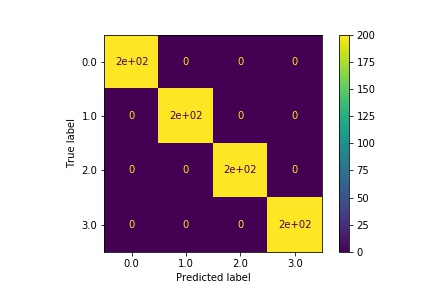
\includegraphics[scale=0.5]{images/1a_cm_knn_train.jpg}
    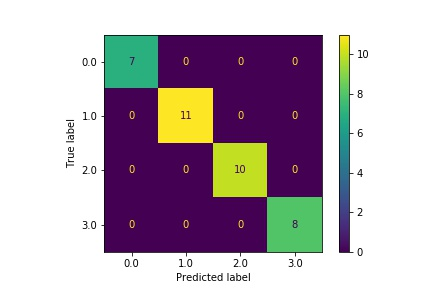
\includegraphics[scale=0.5]{images/1a_cm_knn_test.jpg}
    \caption{Confusion matrix for k=1, Train and Test data set on left and right respectively}
    \label{fig:1a_cm_knn}
\end{figure}

\subsubsection{Decision region plot with training data superposed}

\begin{figure}[H]
    \centering
    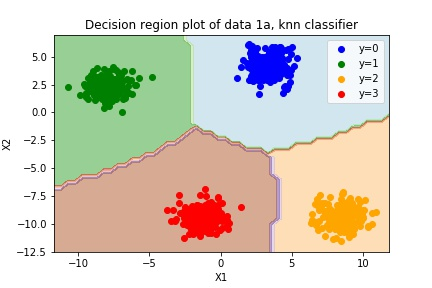
\includegraphics[scale=0.5]{images/1a_knn_decision_region.jpg}
    \caption{Decision region superimposed with training data set}
    \label{fig:1a_decreg_knn}
\end{figure}

The decision boundary obtained (with k=1) is linear in form. 


\subsection{Naive-Bayes classifier with Gaussian distribution for each class}
The Bayes Classifiers are probabilistic classifiers based on the Bayes theorem:

\begin{equation}
\label{eqn nb}
    p(y_{i}/\vec{x})=\frac{p(\vec{x}/y_{i})*p(y_{i})}{p(\vec{x})}
\end{equation}\\

\noi
Here,
\begin{itemize}
    \itemsep0em
    \item $p(y_{i})$ : prior probability for $y=y_{i}$.
    \item $p(\vec{x}/y_{i})$ : Class conditional probability density function or class conditional likelihood function.
    \item $p(y_{i}/\vec{x})$ : Posterior probability for $y=y_{i}$ given $\vec{x}$
    \item $p(\vec{x})$ : Evidence or normalization factor
\end{itemize}

\spa
\noi
Equation \ref{eqn nb} can be re-written as:
\begin{equation} \label{normalized_nb}
    p(y_{i}/\vec{x})=\frac{p(\vec{x}/y_{i})*p(y_{i})}{\sum_{i}p(\vec{x}/y_{i})*p(y_{i})}
\end{equation}\\

\noi
Hence, the probability that $\vec{x}$ belongs to the class $y_{i}$ is $\propto$ $p(\vec{x}/y_{i})*p(y_{i})$.\\

\noi
Step-wise approach:
\begin{itemize}
    \itemsep0em
    \item $p(y_{i})$ is calculated from the train data set, for data set 1a, we find that all the classes have equal prior probability.
    \item The probability $p(\vec{x}/y_{i})$ can be calculated by various parametric and non-parametric means. For data set 1a, we use parametric means as described later.
    \item $p(y_{i}/\vec{x})$ is calculated for all the classes using equation \ref{normalized_nb}.
    \item The class label with maximum posterior probability is chosen as the class label for $\vec{x}$.
\end{itemize}

\noi
For the discussion that follows for data set 1A, we assume that $p(\vec{x}/y_{i})$ is given by a gaussian distribution:

\begin{equation}
\label{gaussian}
    p(\vec{x}/y_{i})=\frac{exp[-(\vec{x}-\vec{\mu_{i}})^{T}*C_{i}^{-1}*(\vec{x}-\vec{\mu_{i}})/2]}{(2\pi)^{d/2}*|C_{i}|^{1/2}}
\end{equation}

\noi
In the above equation: 

\begin{itemize}
    \item $\mu_{i}$ is the mean corresponding to examples in the class $y_{i}$, its dimension is d*1, where d is the number of features. Hence, if there are k classes, number of parameters to be estimated for mean = k*d
    \item $C_{i}$ is the d*d co-variance matrix corresponding to the class $y_{i}$. Since it is symmetric, number of parameters to be calculated per class = $\frac{d(d+1)}{2}$. Total parameters for co-variance = $\frac{k*d(d+1)}{2}$
\end{itemize}

\subsubsection{Case a : Same Covariance Matrix ($\sigma^2I$)}

To reduce the number of parameters to be calculated, we assume that
\begin{equation}
    C_{i}=C_{j}=\sigma^{2}I
\end{equation}
\begin{equation}
\label{casea_nb}
    \sigma^{2}=\frac{\sum_{i=1}^{d}\sum_{k=1}^{K}\sigma^{2}_{ik}}{K*d}
\end{equation}
Where, K is the number of classes (4 for data set 1a) and d is the dimension of feature vector (2 for data set 1a)
\noi
Substituting (\ref{casea_nb}) in equation \ref{gaussian}, $p(\vec{x}/y_{i})$ is calculated and used for predicting the class labels. 
This is also called the naive-bayes classifier since we assume the features to be conditionally independent. 
The decision boundary obtained is linear, while the level curves are circles. 

\subsubsection{Case b : Same Co-variance Matrix ($C$)}

The covariance matrix C is calculated as: 
\begin{equation}
    C=\frac{\sum_{k}^{K}C_{k}}{K}
\end{equation}
Where $C_{k}$ is the co-variance matrix corresponding to the $k^{th}$ class.\\
\noi
With this assumption, the decision boundary is linear, while the level curves are ellipses with equal length of principal axes, proportional to the eigen-vectors of C.

\subsubsection{Case c : Different Co-variance Matrix}

In this case, the decision surfaces are hyper-quadrics.


\subsubsection{Accuracy table and Confusion Matrix}

We obtain that irrespective of our assumption of the co-variance matrices, the accuracy over train, validation and test set is 1. 
\def\arraystretch{1.25}
\begin{center}
\begin{longtable}{l l l l l}
\hline
\hline
\textbf{Assumption} & \textbf{Train Accuracy} & \textbf{Validation Accuracy} & \textbf{Test Accuracy}\\
\hline
\hline
$C_{i}=C_{j}=\sigma^{2}I$ & 1.00 & 1.00 & 1.00\\
$C_{i}=C_{j}=C$ & 1.00 & 1.00 & 1.00 \\
$C_{i}\neq C_{j}$ & 1.00 & 1.00 & 1.00 \\

\hline
\end{longtable}
\setcounter{table}{1}
\captionof{table}{Accuracy table for data set 1a: Bayes Classifier}
\end{center}

\break
\section{Dataset 1B}
\subsection{K Nearest Neighbour Classifier} 

Similar to section \ref{1.1}, K Nearest Neighbour classifier is used to predict class labels for data set 2A. \\The data set 1B has 3 unique class labels - [0.0,1.0,2.0] as shown in the figure, it is also non-linearly separable. The train data set is of dimension (800,3) while the dev data set is of dimension (90,3). Similar preprocessing steps are performed as in section \ref{1.1.1}

\subsubsection{Model performance for varying values of $k$}
Unlike data set 1A, we observe that the accuracy over validation set decreases on increasing the value of hyper-parameter k. This happens because the data set 1B is non-linear, a higher k value includes points from other class labels resulting in mis-judgment.
\\

\noi
The accuracy table is as follows:
\def\arraystretch{1.25}
\begin{center}
\begin{longtable}{l l l l l}
\hline
\hline
\textbf{k-value} & \textbf{Train accuracy} & \textbf{Cross-validation accuracy} & \textbf{Test Accuracy}\\
\hline
\hline
1 & 1.000 & 1.000 & 1.000 \\
7 & 0.995 & 1.00 & 0.978 \\
15 & 0.995 & 1.00 & 0.978 \\

\hline
\end{longtable}
\setcounter{table}{2}
\captionof{table}{Accuracy table for data set 2a- knn classifier}
\end{center}

\noi 
Hence, the best configuration of the model exists for $k=1$.The confusion matrix in this case is:

\begin{figure}[H]
    \centering
    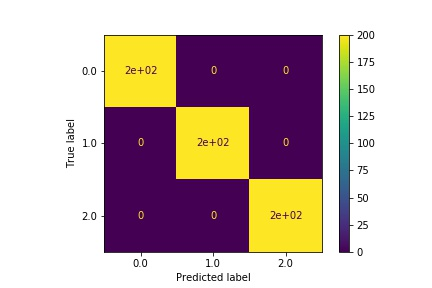
\includegraphics[scale=0.5]{images/1b_cm_knn_train.jpg}
    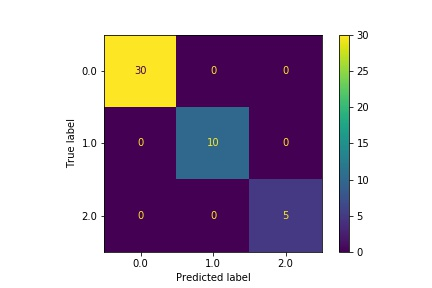
\includegraphics[scale=0.5]{images/1b_cm_knn_test.jpg}
    \caption{Confusion matrix for k=1, for Train and Test data on left and right respectively }
    \label{fig:1b_cm_knn}
\end{figure}

\subsubsection{Decision Boundary plot}

\begin{figure}[H]
    \centering
    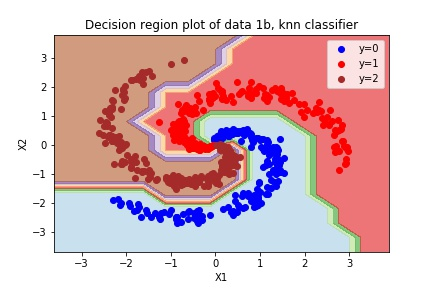
\includegraphics{images/1b_knn_decision_region.jpg}
    \caption{Decision boundary plot for k=1}
    \label{fig:1b_decreg_knn}
\end{figure}

\noi
The decision boundary obtained is non-linear in form and not smooth. 

\subsection{Bayes Classifier, GMM, full covariance}
\subsubsection{Equations}
Th initialization is done as follows for each class:
\begin{itemize}
    \itemsep0em
    \item Cluster initialization is using \tt{kmeans} clustering.
    \item The relative number of points in each cluster $N_q$ and weightage $w_q$ for each cluster is calculated.
    \item The responsibility $\gamma_{n,q}$ is then calculated, followed by mean $\mu_q$ and covariance $C_q$ is calculated.
\end{itemize}

\noi
The parameters are then updated sequentially through the:
\begin{itemize}
    \itemsep0em
    \item Expectation-step: $\gamma_{n,q}$ is updated.
    \item Maximization-step: $\mu_q$, $C_q$, $N_q$ and $w_q$ are updated.
\end{itemize}

\noi
The stopping criterion used is $\Delta(\text{likelihood})<\tt{tol}$. The \tt{tol} we considered is $10^{-5}$.\\

\subsubsection{Training and Validation Accuracy}
The training and validation accuracies obtained for varying $q_i$ for each class is as follows:
\begin{figure}[H]
    \hspace{-2em}
    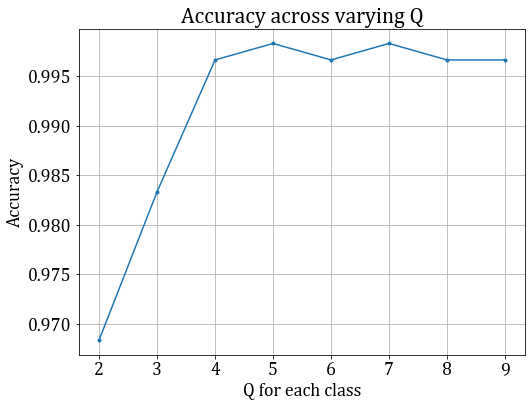
\includegraphics[scale=0.45]{images/1b_full_train.png}
    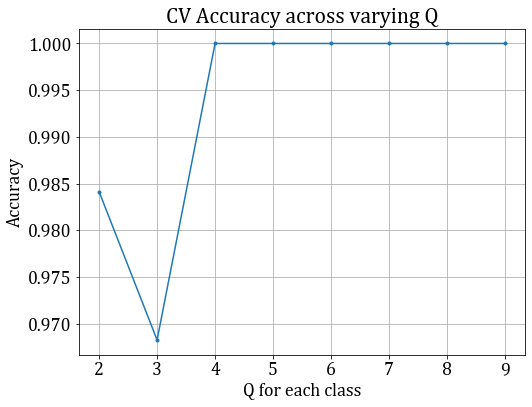
\includegraphics[scale=0.45]{images/1b_full_val.png}
    \caption{Training and Validation accuracy across $q_i$, on the left and right respectively, using a GMM model with full covariance matrix.}
\end{figure}

\subsubsection{Testing Accuracy}
The testing accuracy obtained for varying $q_i$ for each class is as follows:
\begin{figure}[H]
    \centering
    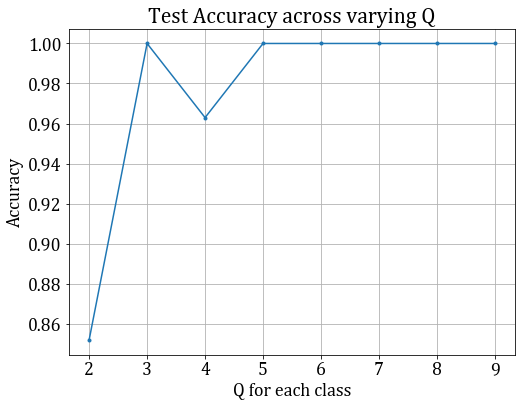
\includegraphics[scale=0.45]{images/1b_full_test.png}
    \caption{Testing accuracy across $q_i$, using a GMM model with full covariance matrix.}
\end{figure}

\subsubsection{Best Model}
Based on the accuracies obtained on the training, validation and test dataset, the best $q_i$ for the three classes has been chosen as $5$. The accuracies obtained in tabular format is as follows:
\begin{table}[H]
\centering
\begin{tabular}{l l l l}
\hline
\hline
\textbf{Number of Clusters/Class (Q)} & \textbf{Train Accuracy} & \textbf{Validation Accuracy} & \textbf{Test Accuracy}\\
\hline
\hline
2 & 0.968333 & 0.952381 & 0.925926 \\
3 & 0.983333 & 0.968254 & 1.000000 \\
4 & 0.996667 & 0.984127 & 1.000000 \\
5 & 0.998333 & 1.000000 & 1.000000 \\
6 & 0.996667 & 1.000000 & 1.000000 \\
7 & 0.998333 & 1.000000 & 1.000000 \\
8 & 0.996667 & 1.000000 & 1.000000 \\
9 & 0.996667 & 1.000000 & 1.000000 \\
\hline
\end{tabular}
\caption{Variation of accuracy across hyperparameter values on the training, validation and test set using the GMM model with full covariance matrix on Dataset 1B}
\label{tab:1b_full}
\end{table}



\noi
The confusion matrix obtained for the model with $q_i=5$ are as follows:
\begin{figure}[H]
    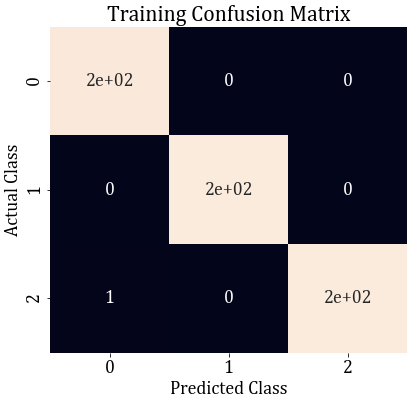
\includegraphics[scale=0.5]{images/1b_full_train_conf.png}
    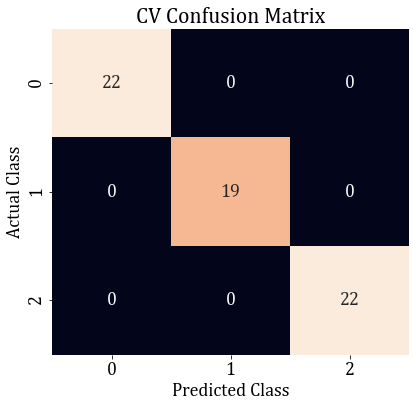
\includegraphics[scale=0.5]{images/1b_full_val_conf.png}
    \caption{Confusion matrices corresponding to training and validation data, with $q_i=5$, on the left and right respectively, using GMM model with full covariance.}
\end{figure}

\begin{figure}[H]
    \centering
    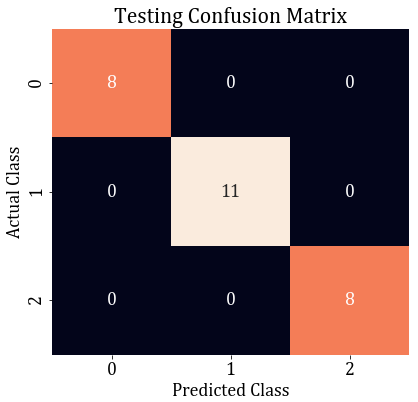
\includegraphics[scale=0.5]{images/1b_full_test_conf.png}
    \caption{Confusion matrix corresponding to the testing data, with $q_i=5$, using GMM model with full covariance.}
\end{figure}

\subsubsection{Contour Maps and Decision Surfaces}
The contour maps and decision surfaces obtained, with $q_i=5$ are as follows:
\begin{figure}[H]
    \hspace{-1em}
    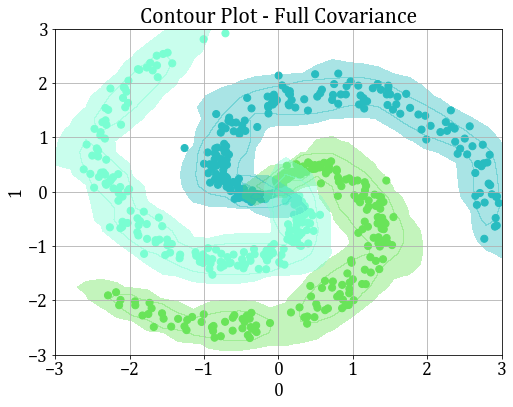
\includegraphics[scale=0.45]{images/1b_full_contours.png}
    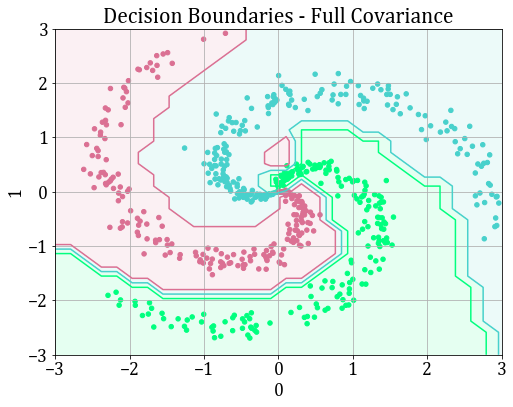
\includegraphics[scale=0.45]{images/1b_full_decision_surfaces.png}
    \caption{Contour Maps, Decision Surfaces obtained for $q_i=5$, on the left and right respectively.}
\end{figure}

\begin{figure}[H]
    \centering
    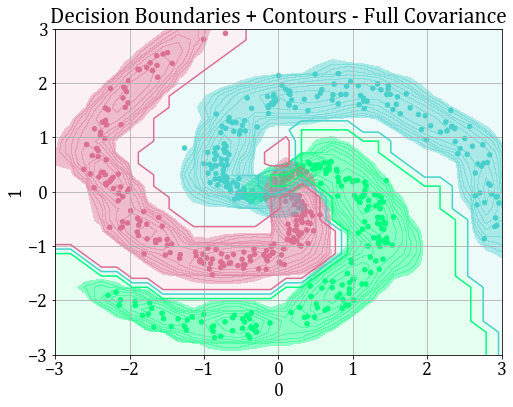
\includegraphics[scale=0.45]{images/1b_full_ds_contours.png}
    \caption{Overlap plot of the decision surface and contours.}
\end{figure}

\subsection{Bayes Classifier, GMM, diagonal covariance}
\subsubsection{Training and Validation accuracy}
Gaussian multi-modal training function (with threshold of the increment in total log-likelihood functions as 0.01) with diagonal covariance matrix over the hyperparameter values of the number of gaussian components Q = {2,3,4,5,6,7,8,9} to estimate the parameters - $\mu_q$, $C_q$, $N_q$ and $w_q$ for each gaussian component - and predict the classes of the training data (train.csv) and cross-validation (70\% of dev.csv), we get the table \ref{tab:cv1b}
\begin{table}[H]
\centering
\begin{tabular}{l l l }
\hline
\hline
\textbf{Hyperparameter Value (Q)} &  \textbf{Accuracy on CV data} &  \textbf{Accuracy on Training data}  \\
\hline
\hline
2 & 0.873 & 0.9166\\
3 & 0.920 & 0.976\\
4 & 0.968 & 0.9966\\
5 & 0.984 & 1.0\\
6 & 0.984 & 0.986\\
7 & 0.984 & 0.991\\
8 & 0.984 & 0.9916\\
9 & 0.984 & 0.9916\\
\hline
\end{tabular}
\caption{Variation of Accuracy across Hyperparameter values on the validation data using the GMM model with diagonal covariance matrix on Dataset 1B}
\label{tab:cv1b}
\end{table}


\begin{figure}[H]
    \centering
    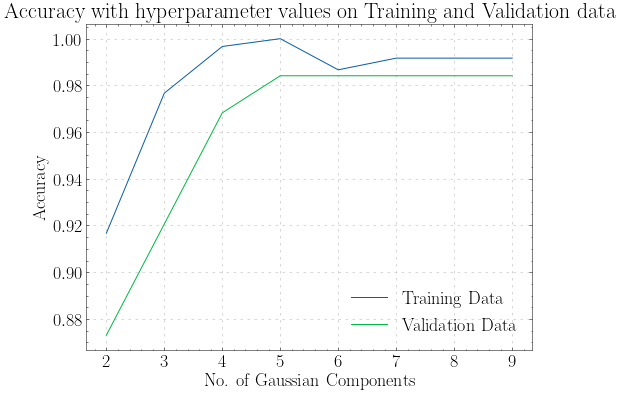
\includegraphics[scale=0.5]{images/acc_1b.png}
    \caption{Training and Validation accuracy across $q_i$, using the GMM model with diagonal covariance matrix on Dataset 1B}
    \label{fig:acc1bGMMdiag}
\end{figure}

\subsubsection{Best model output}
As we can see in the tables and figure \ref{fig:acc1bGMMdiag}, the best accuracy is when the number of Gaussian components is 5. Using the parameters of the model for 5 gaussian components and predicting for the test dataset (30\% of dev.csv), the accuracy obtained was \textbf{1.0}.\\
The confusion matrices for the training and test datasets using the best model is figure \ref{fig:conf_1b_diag}\\
\begin{figure}[H]
    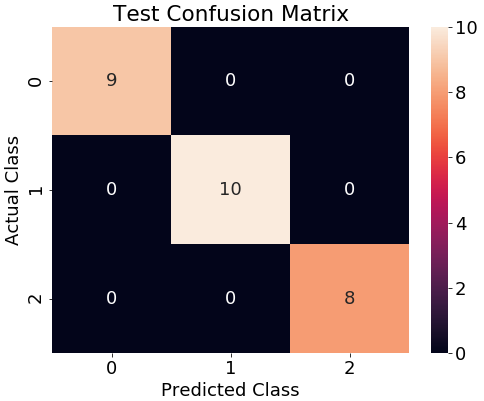
\includegraphics[scale = 0.5]{images/conf_test1b.png}
    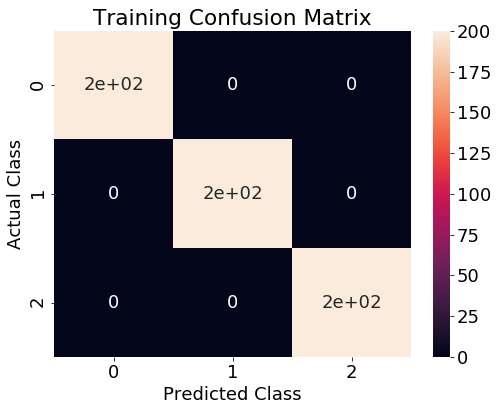
\includegraphics[scale = 0.5]{images/conf_train1b.png}
    \caption{Confusion matrices for data 1B - diagonal covariance matrices}
    \label{fig:conf_1b_diag}
\end{figure}

The decision region plot and the contour plot for the best model is figure \ref{fig:dec1bGMMdiag}
\begin{figure}[H]
    \centering
    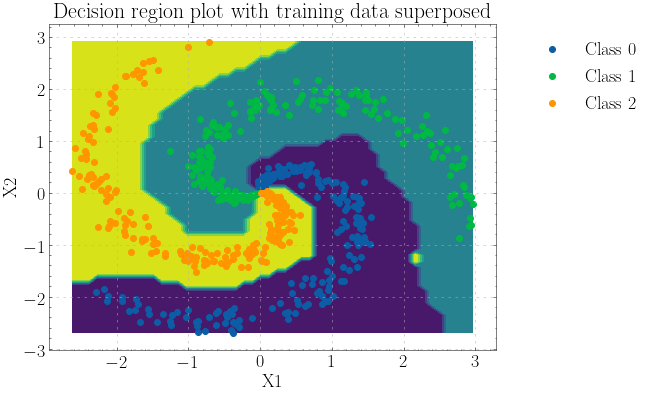
\includegraphics[scale = 0.5]{images/decisionReg_ds2.png}
    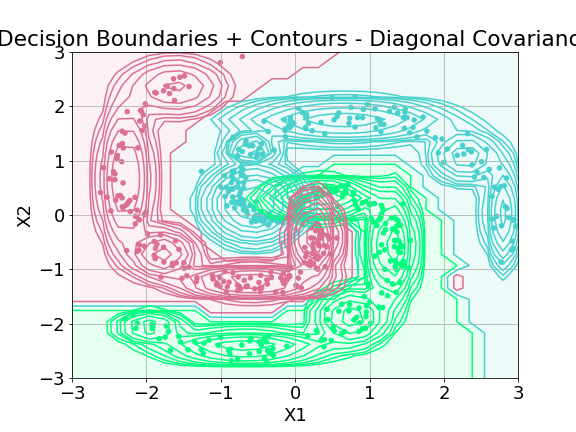
\includegraphics[scale = 0.5]{images/contour1b.png}

    \caption{Decision region plot for Bayesian GMM model using diagonal covariance matrix and 5 gaussian components on dataset 1B}
    \label{fig:dec1bGMMdiag}
\end{figure}

\subsection{Bayes Classifier with KNN}

While the main principle remains the same as discussed in section \ref{1.2}, we now use non-parametric methods to evaluate the class conditional probability $p(\vec{x}/y_{i})$.
\\Suppose the number of data points in the hyper-volume v around $\vec{x}$ be N, the number of data point corresponding to class i be $N_i$, then:

\begin{equation}
    p(\vec{x}/y_{i})=\frac{N_{i}}{N*V}
\end{equation}

The probability density can be estimated in two ways :

\begin{itemize}
    \item Specifying the volume V, number of point $N_i$ and $N$ are calculated
    \item Specifying N, the volume V and $N_i$ are calculated. Here, the radius of hyper sphere is the distance of the point belonging to N farthest from $\vec{x}$, this is called knn method.  
\end{itemize}
\noi
For this case, we use the knn method to evaluate the class conditional probability densities.
\\ 
The class label i that maximizes equation \ref{eqn nb} is chosen as the label for $\vec{x}$. 

\subsubsection{Model Performance for varying values of $k$}
The model is tested for $k=10$ and $k=20$. The accuracy table and confusion matrix are as follows:
\def\arraystretch{1.25}
\begin{center}
\begin{longtable}{l l l l l}
\hline
\hline
\textbf{k-value} & \textbf{Train accuracy} & \textbf{validation accuracy} & \textbf{Test Accuracy}\\
\hline
\hline
10 & 0.991667 & 1.0 & 0.955556 \\
20 & 0.986667 & 1.0 & 0.933333 \\
\hline
\end{longtable}
\setcounter{table}{3}
\captionof{table}{Accuracy table for data set 2a- Bayes Classifier with knn}
\end{center}

\noi
Since the accuracy is higher for $k=10$, it is used to further evaluate the confusion matrix and decision boundary plot. 

\begin{figure}[H]
    \centering
    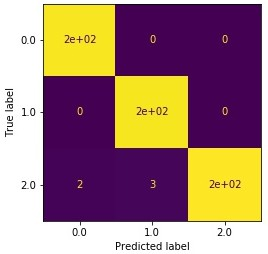
\includegraphics[scale=0.5]{images/1b_cm_nb_train.jpg}
    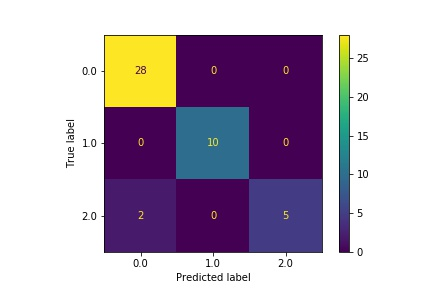
\includegraphics[scale=0.5]{images/1b_cm_nb_test.jpg}
    \caption{Confusion matrices for $k=10$, for train data and test data on left and right respectively.}
    \label{fig:1b_cm_nb}
\end{figure}

\subsubsection{Decision boundary plot}
\begin{figure}[H]
    \centering
    % 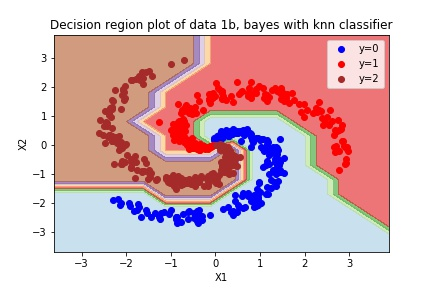
\includegraphics{images/1b_nb_decision_region.jpg}
    \caption{Decision boundary for $k=10$}
    \label{fig:1b_decreg_nb}
\end{figure}
While the shape of decision boundary is almost similar as figure \ref{fig:1b_decreg_knn}, there are still some differences, especially near the edges.

\break
\section{Dataset 2A}
\subsection{Bayes Classifier, GMM, full covariance}
\subsubsection{Training and Validation Accuracy}
The training and validation accuracies obtained for varying $q_i$ for each class is as follows:
\begin{figure}[H]
    \hspace{-2em}
    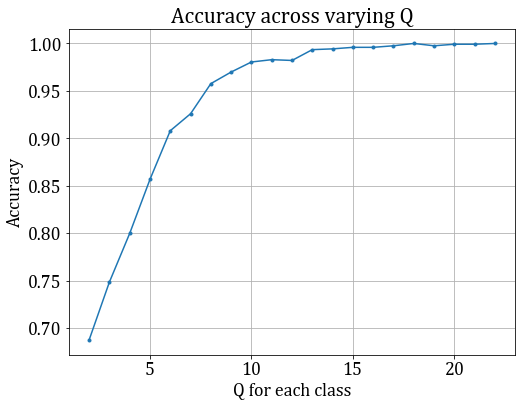
\includegraphics[scale=0.5]{images/2a_full_train_acc.png}
    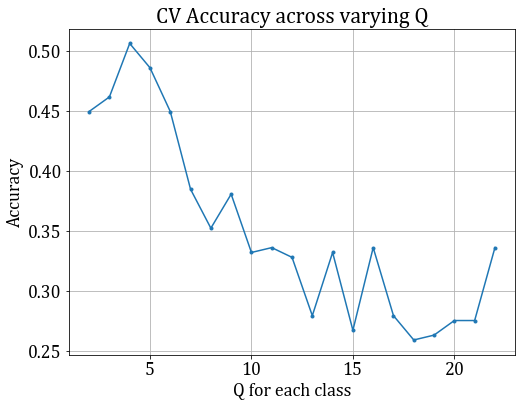
\includegraphics[scale=0.5]{images/2a_full_val_acc.png}
    \caption{Training and Validation accuracy across $q_i$, on the left and right respectively}
\end{figure}

\subsubsection{Testing Accuracy}
The testing accuracy obtained for varying $q_i$ for each class is as follows:
\begin{figure}[H]
    \centering
    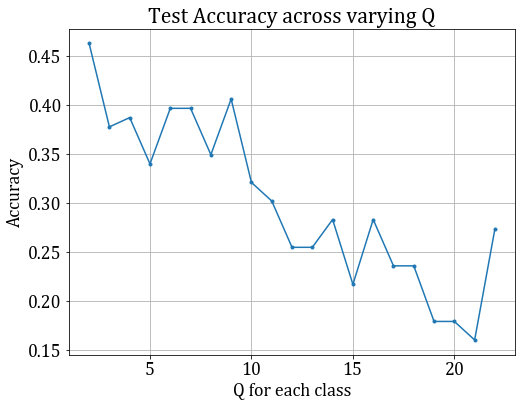
\includegraphics[scale=0.5]{images/2a_full_test_acc.png}
    \caption{Testing accuracy across $q_i$}
\end{figure}

\subsubsection{Best Model}
Based on the accuracies obtained on the training, validation and test dataset, the best $q_i$ for the three classes has been chosen as $6$. The accuracies obtained in tabular format is as follows:
\begin{table}[H]
\centering
\begin{longtable}{l l l l l}
\hline
\hline
\textbf{\# Clusters/Class (Q)} & \textbf{Train Accuracy} & \textbf{Validation Accuracy} & \textbf{Test Accuracy} & \textbf{Sum(Train,Validation)} \\
\hline
\hline
2 & 0.687805 & 0.449393 & 0.462264 & 1.137198 \\
3 & 0.748780 & 0.461538 & 0.377358 & 1.210319 \\
4 & 0.800000 & 0.506073 & 0.386792 & 1.306073 \\
5 & 0.856911 & 0.485830 & 0.339623 & 1.342741 \\
6 & 0.908130 & 0.449393 & 0.396226 & 1.357523 \\
7 & 0.926016 & 0.384615 & 0.396226 & 1.310632 \\
8 & 0.957724 & 0.352227 & 0.349057 & 1.309950 \\
9 & 0.969919 & 0.380567 & 0.405660 & 1.350486 \\
10 & 0.980488 & 0.331984 & 0.320755 & 1.312472 \\
11 & 0.982927 & 0.336032 & 0.301887 & 1.318959 \\
12 & 0.982114 & 0.327935 & 0.254717 & 1.310049 \\
13 & 0.993496 & 0.279352 & 0.254717 & 1.272848 \\
14 & 0.994309 & 0.331984 & 0.283019 & 1.326293 \\
15 & 0.995935 & 0.267206 & 0.216981 & 1.263141 \\
16 & 0.995935 & 0.336032 & 0.283019 & 1.331967 \\
17 & 0.997561 & 0.279352 & 0.235849 & 1.276913 \\
18 & 1.000000 & 0.259109 & 0.235849 & 1.259109 \\
19 & 0.997561 & 0.263158 & 0.179245 & 1.260719 \\
20 & 0.999187 & 0.275304 & 0.179245 & 1.274491 \\
21 & 0.999187 & 0.275304 & 0.160377 & 1.274491 \\
22 & 1.000000 & 0.336032 & 0.273585 & 1.336032 \\
\hline
\end{longtable}
\caption{Variation of accuracy across hyperparameter values on the training, validation and test set using the GMM model with full covariance matrix on Dataset 2A}
\label{tab:1b_full}
\end{table}



\noi
The confusion matrix obtained for the model with $q_i=6$ are as follows:
\begin{figure}[H]
    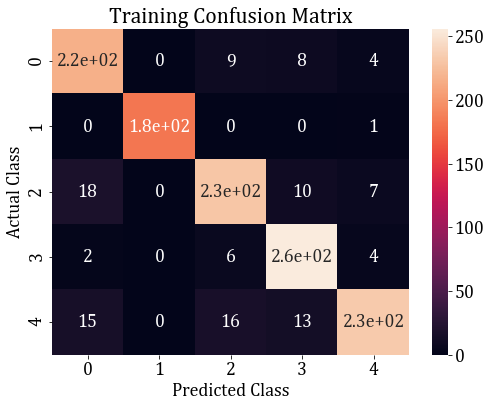
\includegraphics[scale=0.5]{images/2a_full_train_conf.png}
    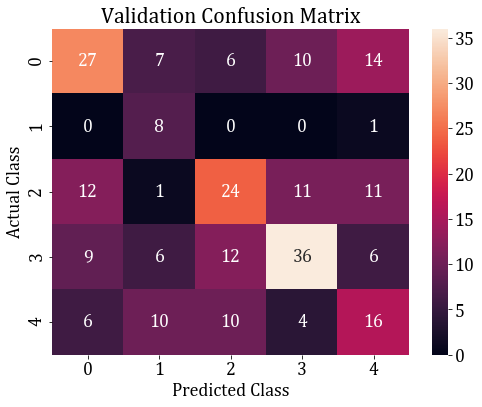
\includegraphics[scale=0.5]{images/2a_full_val_conf.png}
    \caption{Training and Validation confusion matrices for the best model with $q_i=6$, on the left and right respectively}
\end{figure}

\begin{figure}[H]
    \centering
    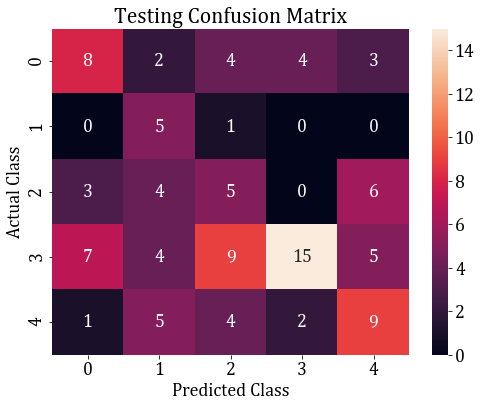
\includegraphics[scale=0.5]{images/2a_full_test_conf.png}
    \caption{Testing confusion matrix for the best model with $q_i=6$.}
\end{figure}

\noi
In addition to just taking the same number of clusters for all classes, a parameter sweep was done to identify the best combination of cluster numbers for the dataset. The accuracies obtained from the parameter sweeps are as follows:
\begin{figure}[H]
    \centering
    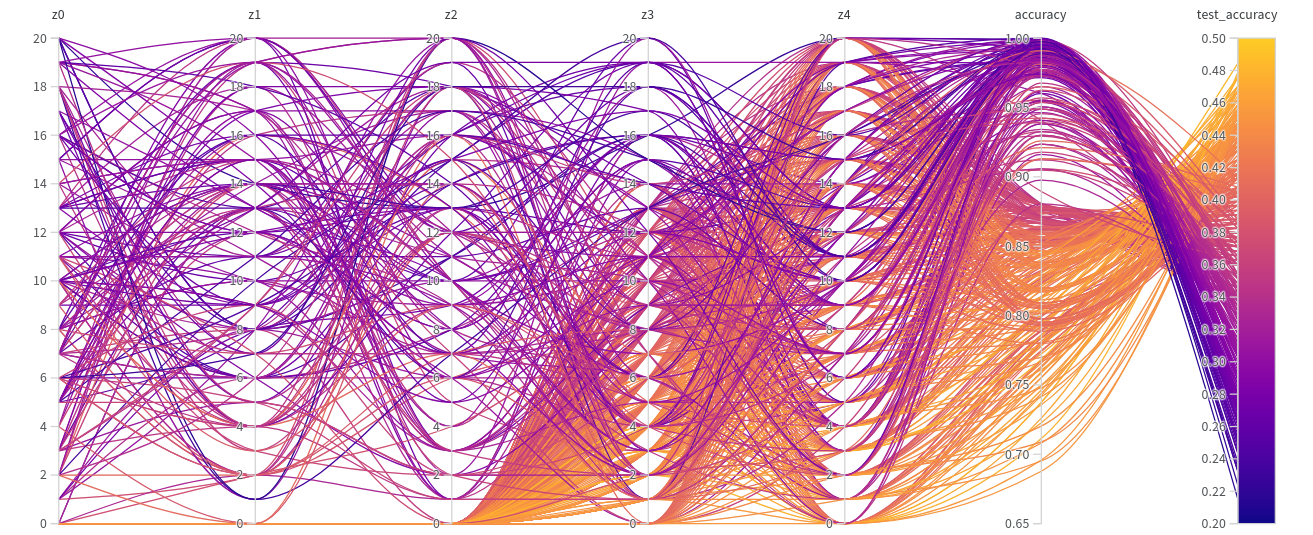
\includegraphics[scale=0.35]{images/2a_parameter_sweep.png}
    \caption{Parameter Sweep Results for the dataset 2A.}
\end{figure}

\noi
From the graph above, the parameter combination that resulted in the best validation accuracy is:
\begin{itemize}
    \itemsep0em
    \item $q_1: 2$
    \item $q_2: 2$
    \item $q_3: 2$
    \item $q_4: 6$
    \item $q_5: 3$
\end{itemize}

\noi
The accuracies obtained are as follows:
\begin{itemize}
    \itemsep0em
    \item Training accuracy: 0.7853658536585366
    \item Validation accuracy: 0.4939271255060729
    \item Testing accuracy: 0.46226415094339623
\end{itemize}

\noi
From the results above, we can see that the validation and test accuracies are higher in this case, however, the train accuracy is low.\\

\noi
The confusion matrices obtained are as follows:
\begin{figure}[H]
    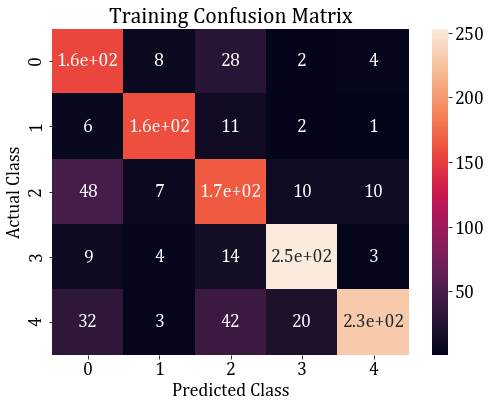
\includegraphics[scale=0.5]{images/2a_full_cross_train.png}
    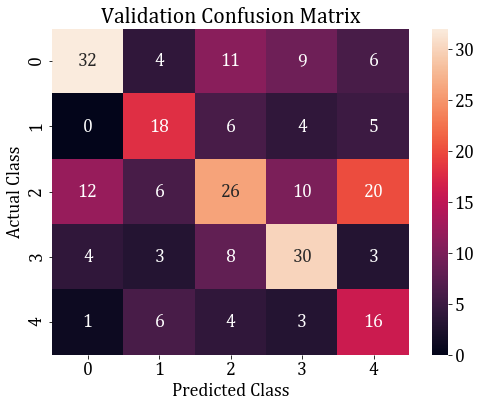
\includegraphics[scale=0.5]{images/2a_full_cross_val.png}
    \caption{Training and Validation confusion matrices for the model with varying $q_i$, on the left and right respectively}
\end{figure}

\begin{figure}[H]
    \centering
    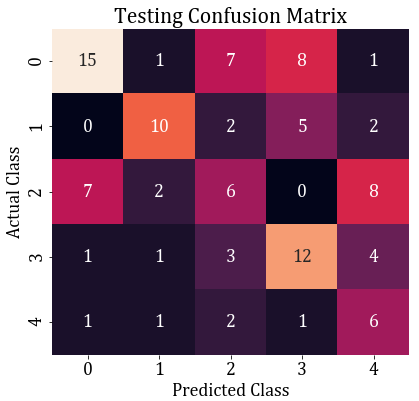
\includegraphics[scale=0.5]{images/2a_full_cross_test.png}
    \caption{Testing confusion matrix for the model with varying $q_i$.}
\end{figure}


\subsection{Bayes Classifier, GMM, diagonal covariance}
\subsubsection{Training and Validation Accuracy}
The accuracy obtained on training the data 2A on GMM model with diagonal covariance matrix is as in table \ref{tab:acc2a}. The plot of the same is in figure \ref{fig:acc2adiag}. The tolerance used was 1e-3.
\begin{table}[H]
\centering
\begin{tabular}{l l l l}
\hline
\hline
\textbf{# Clusters/Class (Q)} & \textbf{Training Accuracy} & \textbf{Validation Accuracy}\\
\hline
\hline
2 & 0.509 & 0.350\\
3 & 0.525 & 0.404\\
4 & 0.574 & 0.436\\
5 & 0.627 & 0.420\\
6 & 0.6491 & 0.418\\
\hl{7} & \hl{0.663} & \hl{0.440}\\
8 & 0.689 & 0.371\\
9 & 0.692 & 0.413\\
10 & 0.718 & 0.427\\
11 & 0.735 & 0.396\\
12 & 0.754 & 0.393\\
13 & 0.770 & 0.434\\
14 & 0.783 & 0.388\\
\hline
\end{tabular}
\caption{Variation of accuracy across hyperparameter values on the training and validation using the GMM model with diagonal covariance matrix on Dataset 2A. }
\label{tab:acc2a}
\end{table}



\begin{figure}[H]
    \centering
    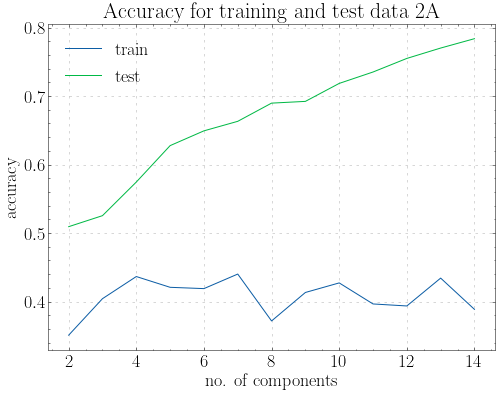
\includegraphics[scale = 0.5]{images/acc_2a.png}
    \caption{Accuracy for training and validation set for 2A}
    \label{fig:acc2adiag}
\end{figure}

\subsubsection{Best model on test data}
The highest accuracy on validation data set is for 7 gaussian components. Applying this model to predict the test data, we get an accuracy of \textbf{0.37}. The confusion matrices for this model on training and test data is figure \ref{fig:conf_2a_diag} .
\begin{figure}[H]
    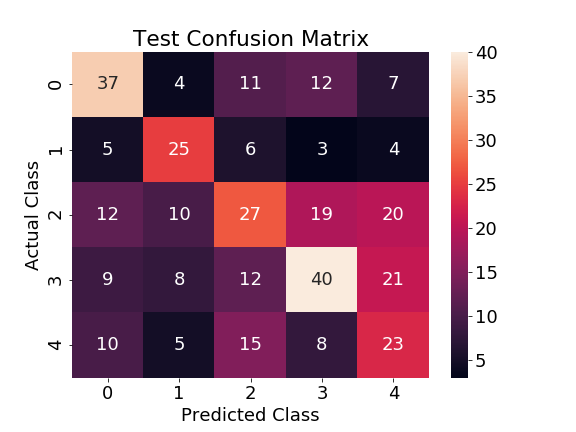
\includegraphics[scale = 0.5]{images/conf_test2a.png}
    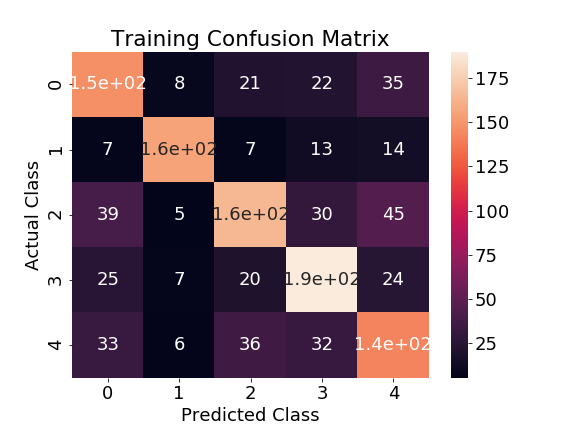
\includegraphics[scale = 0.5]{images/conf_train2a.png}
    \caption{Confusion matrices for data 2A - diagonal covariance matrices}
    \label{fig:conf_2a_diag}
\end{figure}


\break
\section{Dataset 2B}
The varying length classification is done as follows:
\begin{itemize}
    \itemsep0em
    \item Each image has a $36*23$ feature parameters.
    \item Each of these $36$ rows are considered as instances of the class and a GMM (full covariance/diagonal covariance) is fit on the dataset.
    \item The E-step and M-step are done as is in case of static length pattern.
    \item However, for each of these images, 
    \begin{equation}
    p (X|\lambda_i ) = \prod_{t=1}^T p(x_t|\lambda_i) = \prod_{t=1}^T \sum_{q=1}^Q w_{iq}\mathcal{N}(x_t|\mu_{iq}, \Sigma_{iq})
    \end{equation}
    is calculated to perform classification.
\end{itemize}

\noi
Due to the size of the dataset, we weren't able to completely train the models of the five classes. 
\end{document}
